%! Author = NekoHitDev
%! Date = 2021/7/30
%! Language = English (US)
%! compiler = XeLaTex

% Preamble
\documentclass[12pt,a4paper]{article}
\usepackage[T1]{fontenc}

% Packages
\usepackage{amsmath}
\usepackage{url}
\usepackage{graphicx}
\usepackage[slantfont, boldfont]{xeCJK}

% set CJK font
\setCJKmainfont{SimSun}

% include header file
\newcommand{\editversion}{v0.0.1-RC1}

\newcommand{\gentitlepage}[1]{
    \begin{titlepage}
        \centering
        \vfill
        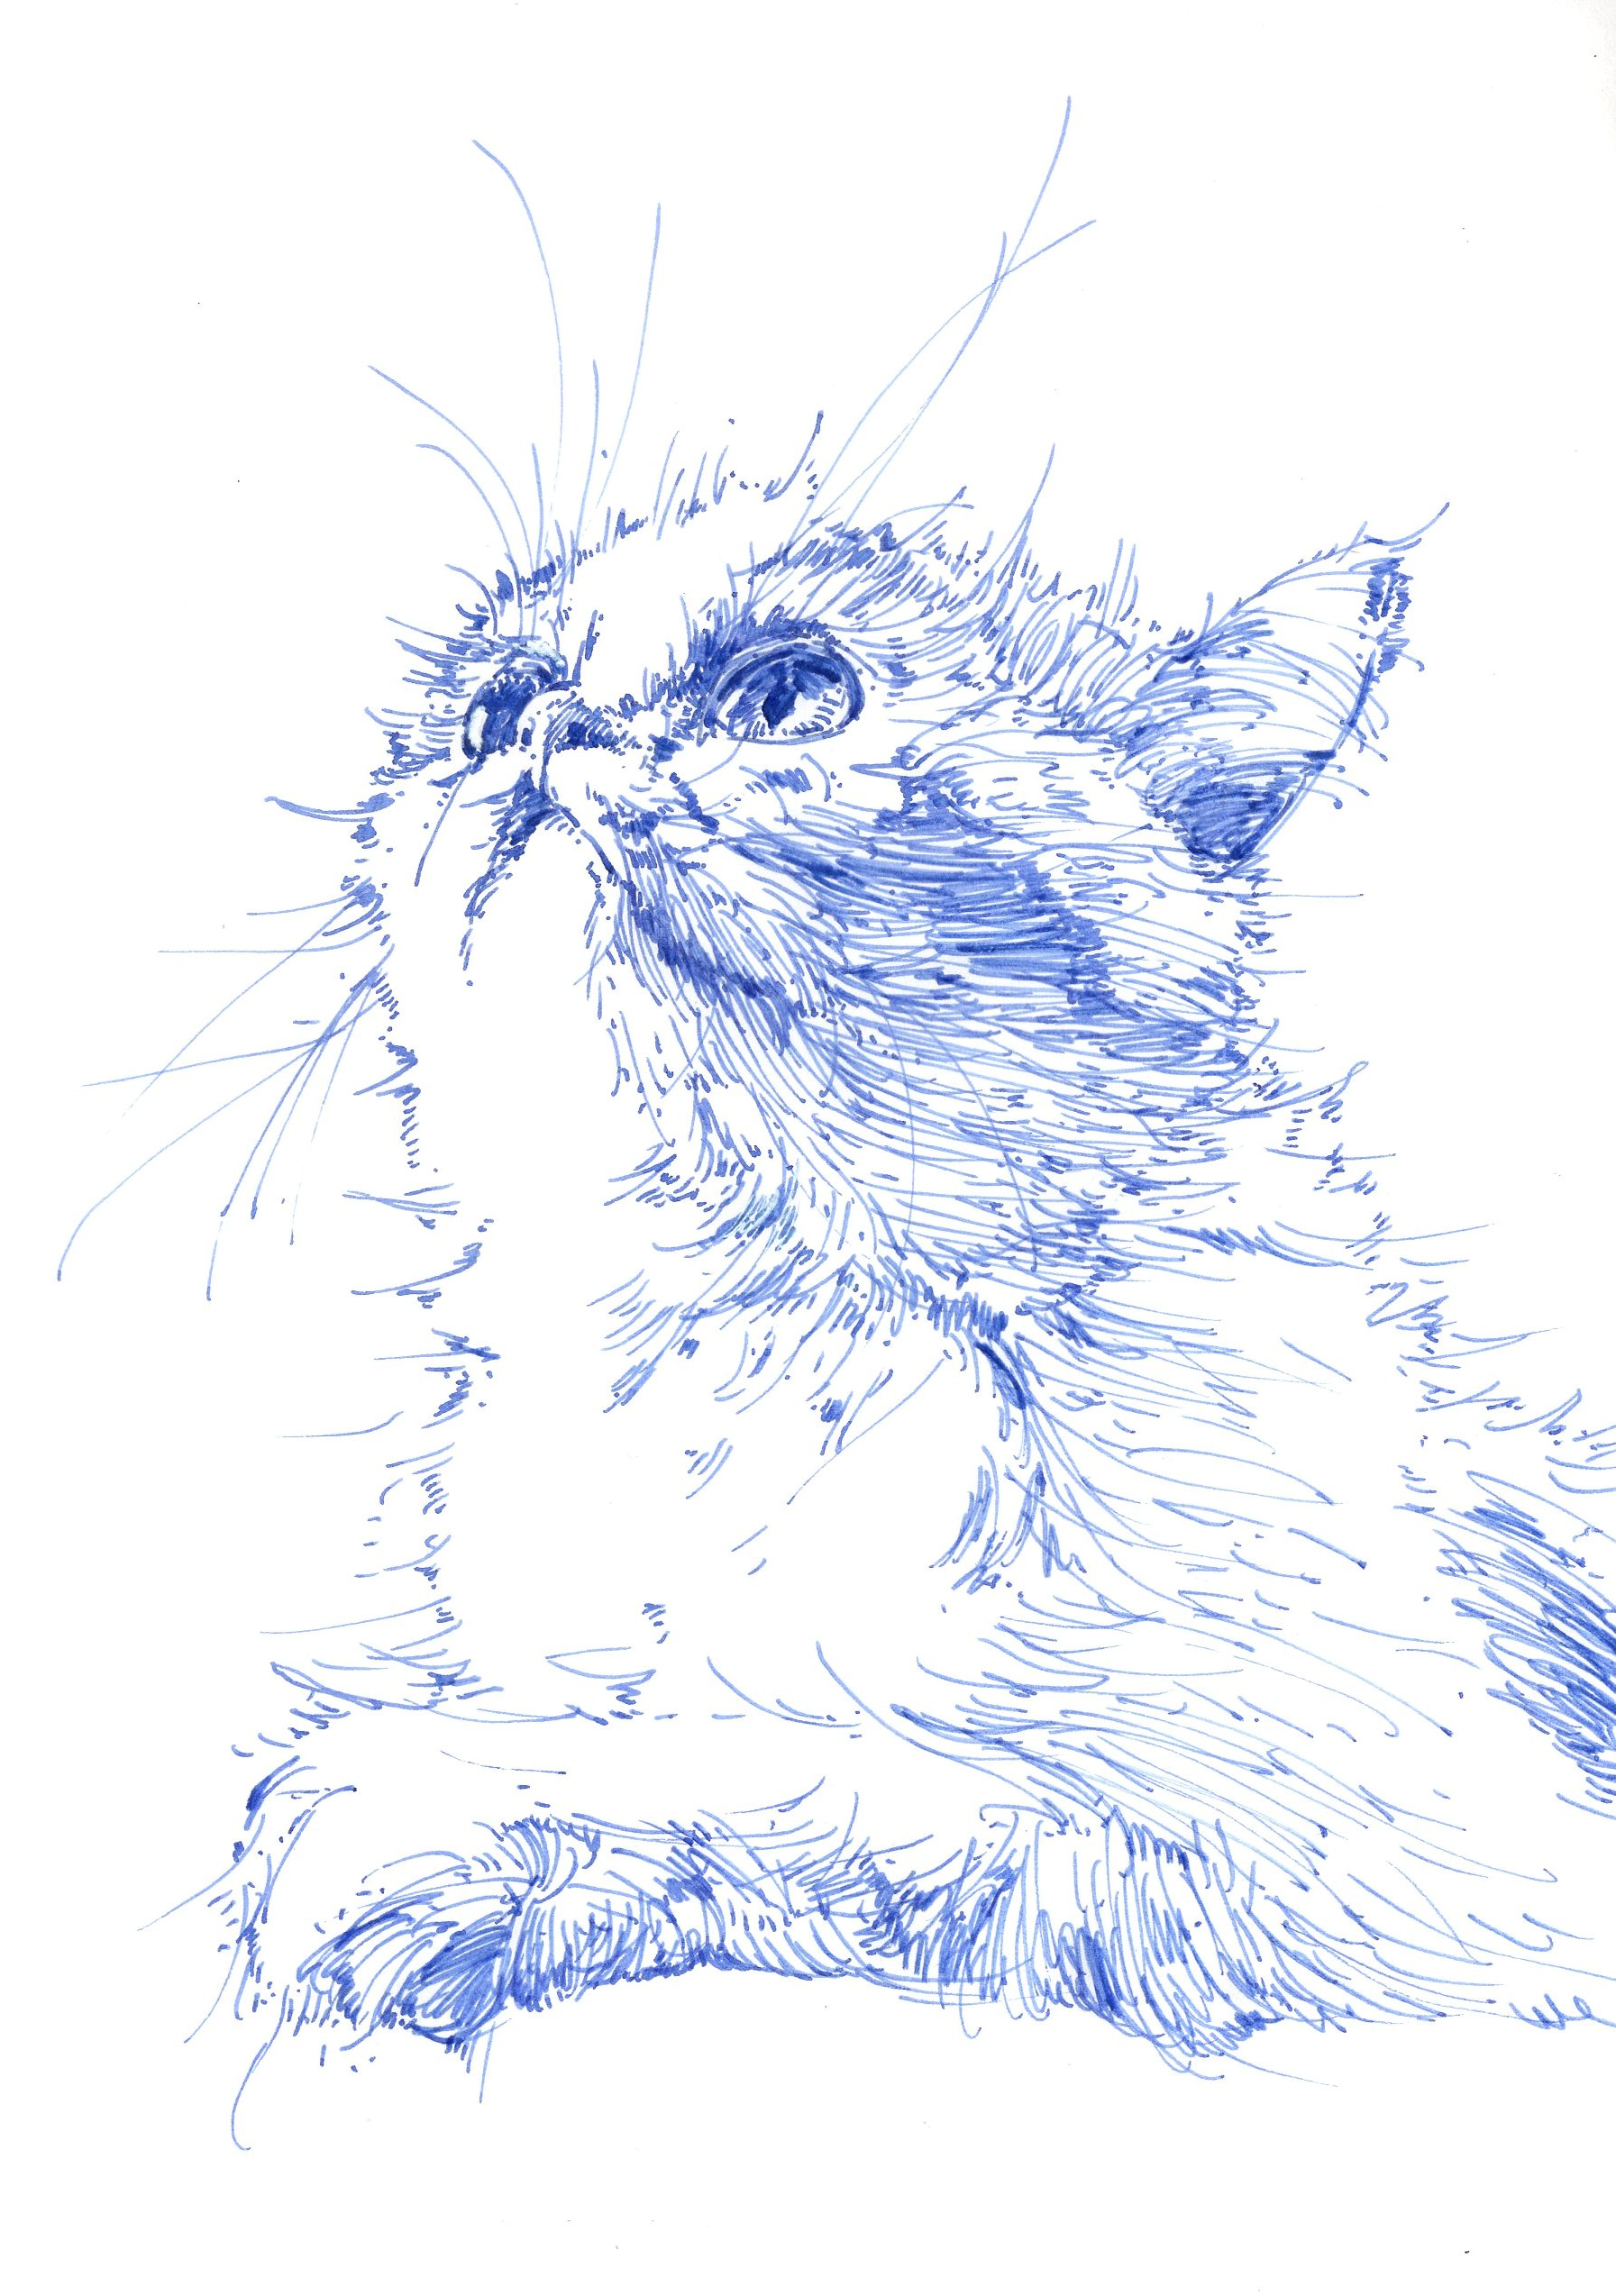
\includegraphics[width=0.8\textwidth]{assets/img196}
        \vfill
        {\Huge
        \textsf{NekoHit Project}\\
        #1\\
        \vskip2cm
        \vfill
        \Large
        \editversion
        }
        \vfill
        \vfill
    \end{titlepage}
}

% TOC stop at subsection
\setcounter{tocdepth}{2}


% Document
\begin{document}
    \gentitlepage{White paper}
    \pagenumbering{Roman}
    \tableofcontents
    \vspace*{\fill}
    \begin{center}
        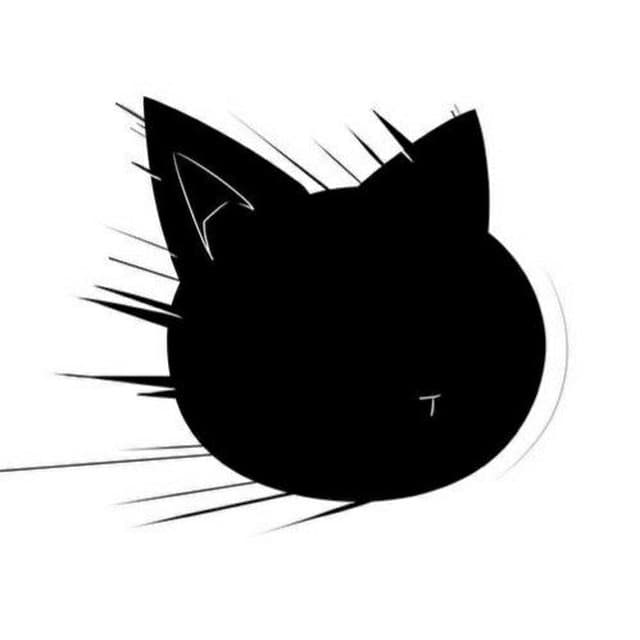
\includegraphics[width=0.67\textwidth]{assets/img197}
    \end{center}
    \clearpage

    \pagenumbering{arabic}


    \section{Goal}\label{sec:goal}

    The goal of the NekoHit Project is to build a decentralized application
    that allows audiences to support creators economically, while motivating
    creators to respond to the sponsors.

    We envisioned: With the addition of more and more creators and sponsors,
    the NekoHit community will gradually grow and improve.
    We, as developers of the app, will work with the community and respond
    to the needs and feedback from the community users, to create an
    energetic platform for creators.


    \section{Introduction}\label{sec:intro}

    The NekoHit Project built on creator work completion agreement
    ("WCA" for short), briefly says that it is the blockchain version
    of Patreon.
    The project aims to incorporate "insurance" into traditional sponsor
    patterns.
    Thus, to promote the willingness of audiences to provide economic
    support for content creators, and motivate creators to comply with their promises
    and get the project finished on time.

    The subscription model of the NekoHit Project is different from Patreon.
    We allow sponsors to be able to sponsor a project more specifically,
    instead of paying a monthly subscription fee.
    In order to gain the trust of readers with the audience,
    content creators need to pledge (stake) some tokens first.
    These tokens need to be transferred to our WCA smart contracts
    before the sponsors can transfer the tokens for sponsorship to
    the creators' projects.
    The sponsored tokens are also held by our WCA contract.
    When declaring a project, the creator needs to provide information such as
    the rate of the pledging, the detailed milestones of the project and
    the expected completion time.
    If the creator fails to complete certain milestones before the expected time,
    WCA contract will automatically calculate the amount corresponding to these milestones
    and deduct from the creator's pledge.
    Upon completion of the project, the deducted tokens will be issued to
    each of the sponsors based on their sponsored amount.
    Also, the sponsored tokens will deduct the corresponding proportion,
    as a refund and returned to the Sponsor's wallet.
    So the creator not only won't receive the part of sponsored tokens,
    but also lost some of his own pledge.

    We use this mechanism as a safety net to protect the interests of sponsors,
    and use this as an incentive for creators to complete projects as expected.
    Such a mechanism will also urge the creators to think about the process
    of the project and arrange a suitable timeline when they create the project.
    Finally, we want to be able to increase the trust of supporters towards
    content creators, and reduce their concerns when carrying out
    economic sponsorships.


    \section{Industry Status}\label{sec:now}

    The "creator economy" is getting more and more attention at the moment,
    with audiences not only willing to fund creators, but creators also
    need various channels to get revenue to maintain their creations.
    The market of the creator's economy is still in a more primitive state,
    and this is undoubtedly an opportunity for our development.


    \subsection{Traditional subscription}\label{subsec:tradition_patreon}

    基于订阅的传统模式,最典型的就是Patreon和爱发电。他们基于按月订阅的模式,创作者可以
    自定义不同金额的计划,通常较低金额的计划享有的回报较少。以著名画师WLOP为例,他的Patreon
    分为五种计划\cite{wlop_patreon}:
    \begin{itemize}
        \item Knight:每月2美元,可以获得JPG格式鬼刀漫画(3000像素宽),及当月创作的壁纸(4K分辨率)
        \item Black Knight:每月4美元,可以获得全尺寸的鬼刀漫画,及当月创作的壁纸(8K分辨率)
        \item Templar:每月8美元,除了Black Knight的内容外,还可以获得画师在Photoshop中使用的笔刷,及当月创作的PSD源文件。
        \item Angel:每月14美元,除了Templar的内容外,在画师自营的商店中获得40\%的优惠,或动态版的壁纸,以及绘画过程的原始录像(1080P,无倍速),以及当月面向绘画初学者的基础教程,同时购买以往教程时享受40\%的优惠。
        \item Asura:每月20美元,除了Angel的内容外,每月可免费获得任意以往作品、教程或动态壁纸的源文件。
    \end{itemize}\footnote{WLOP的Patreon是按Term收费,每月两2个Term,表中定价为月度费用。}

    截至2021年7月30日,画师WLOP在Patreon上共有5854名赞助者,并保持平均每月两到三次的更新频率。
    然而并非所有创作者都能复刻WLOP在Patreon的成功。 我们再来看Sonic Ether的Patreon。
    Sonic Ether是Minecraft著名光影包SEUS的作者,目前他正在制作Minecraft Java版的光追光影。
    他的Patreon有四种计划\cite{seus_patreon}:
    \begin{itemize}
        \item Stone:每月1美元,可以加入Discord服务器并拥有Stone权限,并获取最新开发进度与截图。
        \item Iron:每月5美元,除了Stone的内容之外,在服务器中拥有Iron权限。
        \item Gold:每月10美元,除了Iron的内容之外,在服务器中拥有Gold权限。
        \item Diamond:每月25美元,除了Gold的内容之外,在服务器中拥有Diamond权限。
    \end{itemize}

    截至2021年7月30日,Sonic Ether在Patreon上共有6923名赞助者,并保持平均每两到三个月一次更新的频率。
    值得一提的是,在2021年7月22日,Sonic Ether将以往需要每月订阅Gold计划才能获得的开发版本光影包修改为
    所有人都可以获得,不再需要每月赞助。目前Sonic Ether每月可获得56939美元的收入。

    在这两个例子中,都是创作者先发布作品,然后转向Patreon\footnote{
        Sonic Ether在2017年10月14日开始使用Patreon,而光影包则在2016年开始发布。
        WLOP在2015年1月15日才开始使用Patreon,但他早在2014年就开始发布作品了。
    }。这就要求使用Patreon的创作者,首先有卓越的作品,其次有稳定且合理的更新频率,
    才有可能获得实现赞助支撑创作。而对于刚刚起步,或诸如硬件等其他不便于交付的成果,
    创作者们更多使用众筹的模式。

    \subsection{Traditional crowdfunding}\label{subsec:tradition_kickstarter}

    相比于每月付费的Patreon,基于众筹的传统模式,以Kickstarter为例,则更倾向于一次性
    赞助的方式。在Kickstarter的网站上,可以看到各种各样的众筹类型\cite{kickstarter_homepage},
    包括艺术展览、漫画插图、设计、影片、视频工艺、游戏、硬件、音乐、出版等等各种各样的众筹项目。

    根据Kickstarter自己的介绍\cite{kickstarter_about},该平台致力于将创意转换为现实。
    众筹项目的发起人将对作品具有完全的控制权,并且发起众筹项目相对容易:不需要几百页的项目申请
    书,也不会有捐款者要求对项目做出修改,更不会出现投资者在最终时刻要求修改产品的情况。
    总的来说,Kickstarter更偏向于服务创作者,给他们尽可能多的自由以使他们能够将优秀的创意
    转换为现实中的产品。这种创作者的独立性能够激发出卓越的产品,可一旦遇到恶意项目,当赞助者
    发现他们上当了的时候,他们几乎做不了什么。

    以Milk Nanny为例\cite{kickstarter_milk_nanny},该项目的宣传为一款智能冲奶机。
    使用时只需要打开手机APP,输入小孩的出生年月,再扫一下奶粉的条码,便可以自动冲泡,耗时不到一分钟。
    该项目筹集到了12万美元,但从该项目的留言来看,产品并没有兑现,赞助者们既没有得到冲奶机,
    也没有得到退款。

    同样烂尾的还有Cabin项目\cite{kickstarter_cabin},该项目宣传为一种最方便的为iPhone充电的
    方式。该项目收到了18万8千多美元,只有一小部分赞助者在晚于预定时间8个月后收到了产品,但其中不少人
    反馈无法像宣传的那样使用。而其他赞助者再也没有收到产品,并且该项目在Kickstarter上也没有了更新。

    \subsection{Summary for traditional methods}\label{subsec:tradition_summary}

    基于众筹的传统模式将主动权全部放在了创作者身上,一旦赞助者支付了赞助钱款,该钱款会直接进入
    创作者的账户,之后项目能否完成,赞助者能否得到产品或退款,则完全听天由命。而基于每月订阅
    的传统模式,虽然赞助者可以选择下月起停止订阅,但对于已经订阅计划的赞助者来说,创作者就算什么
    也不做,什么也不更新,他们能做的也只有停止下月的付款。

    然而随着区块链技术以及加密货币逐渐出现在公众视野中,也有人尝试在区块链上实现创作者经济。

    \subsection{瞬matataki}\label{subsec:blockchain_matataki}

    瞬matataki平台意图帮助自由的创作者获得更多收入并建立公开永存的数字作品库。
    该平台提出Fan票和个人通证的概念。Fan票基于以太坊Rinkeby测试网络构建,每个人
    都可以再平台上发行属于自己的Fan票,这些Fan票可以被其他人持有和消费
    (用于解锁发行者的文章)\cite{mitataki_fan_ticket}。

    该平台主打作者自由创作。通过在该平台上发行个人代币,读者可通过
    法定货币兑换创作者的代币,并在未来通过该代币购买创作者作品的阅读权限。同时
    该平台将创作者的作品存储于IPFS\cite{ipfs}上,做到了内容的去中心化存储,
    避免了潜在的内容审查。

    灵活的货币模型给予了瞬matataki平台更多的可能性,但我们认为过于灵活多变的货币
    模型会给内容创造者带来不必要的负担。并且目前来看除了平台本身之外,尚且没有办法
    越过平台直接与以太坊Rinkeby测试网络或IPFS节点交互并使用平台的方法。并且该平台
    的无手续费交易依赖于Rinkeby测试网,迁移到以太坊主网将会导致每笔交易产生高额
    手续费,进而阻碍用户在平台上使用个人代币进行小额交易。但停留在测试网络需要
    平台为个人代币的价值提供担保。


    \section{Our solution}\label{sec:solution}

    上一节中我们列举了两个传统应用和一个基于区块链构建的平台。我们总结了这三种模式的优缺点,
    并提出了NekoHit Project。该企划由两个关键部分组成:作品完成度协议(WCA)和完成
    协议代币(CAT)。我们的企划注重实现一个简单便捷好用的赞助平台,并且给予用户(创作者和
    赞助者)充分保护自己权益的权力与能力。同时我们尽可能保持开放:我们并不限制创作者使用
    何种平台存放作品,也不限制用户以何种方式调用我们的合约,在未来我们还将尽力实现用户的代币
    自由,即不限制用户使用何种代币进行质押与赞助。

    \subsection{Work complete agreement}\label{subsec:wca}

    作品完成度协议(WCA)是NekoHit Project的核心功能。WCA以项目为基本单位,兼具Kickstarter众筹
    与Patreon赞助的功能,并且在传统模式的基础上赋予赞助者更多主动权,除了可以随时退款\footnote{
        退款取决于项目的进行进度,在某些情况下无法全额退款
    }之外,还提供类似保险的机制,在创作者未能如期完成约定时将自动退款至赞助者的钱包,并对创作者做出惩罚。
    以下将对WCA和具体机制进行详细解释。

    \subsubsection{使用流程总览}

    WCA的一次完整使用流程如下:

    \begin{enumerate}
        \item 创作者调用WCA合约声明项目
        \item 创作者调用CAT合约转账(质押代币)
        \item 读者或观众调用CAT合约转账(赞助项目)\label{item:purchase_wca}
        \item 创作者调用WCA合约更新项目进度(更新里程碑)\label{item:update_milestone}
        \item 创作者或赞助者调用WCA合约进行项目结算(结束项目)\label{item:finish_project}
    \end{enumerate}

    其中步骤\ref{item:update_milestone}可由创作者多次调用,以更新不同的里程碑。
    赞助者可以从步骤\ref{item:purchase_wca}转账赞助的一刻开始,到步骤\ref{item:finish_project}
    项目结束前随时退款,但退款数额依照项目进行情况,可退款的金额从全额到部分不等。

    \subsubsection{声明项目}

    声明项目是指将给定的项目信息与全网唯一的标识符绑定,并存储到WCA合约的存储区中。
    声明项目是要求的信息如下:

    \paragraph{创作者的ScriptHash}

    ScriptHash由Neo N3钱包地址的生成,每一个地址对应唯一的ScriptHash,可以理解为面向合约的N3钱包地址。
    合约需要追踪该地址以确认更新等操作只能由合约的创建者调用。

    \paragraph{项目简介}

    对项目的简单介绍。需要注意的是存储在Neo N3区块链上的每一字节数据都需要支付Gas,所以请尽量做到言简意赅,
    或给出链下的项目介绍URL、IPFS CID等链接。

    \paragraph{质押比率}

    决定了质押的总额度,也是违约时赔付的比率。

    \paragraph{最大赞助数额}

    决定了总赞助金额的上限。所有赞助者对项目的赞助数据不能超过该值。

    \paragraph{里程碑列表}

    是项目里程碑的具体定义。每个里程碑有三个字段:标题、简介和预期完成时间。其中预期完成时间使用时间戳存储,
    最大精度可达到毫秒级别。在众多里程碑中,有一个里程碑是特殊的里程碑,即由用户指定的阈值里程碑。
    对于所有里程碑,要求前一个里程碑的预期完成时间总早于后一个。

    \paragraph{阈值里程碑}

    该里程碑决定了赞助者退款时合约结算的行为。若在此里程碑完成之前申请退款,赞助者可以得到全额退款。
    若在此里程碑完成后申请退款,则只能退回作者尚未完成的里程碑所对应的比例,并且无法获得作者对于
    未完成里程碑的惩罚。

    \paragraph{更新冷却时间}

    该值决定了两次里程碑更新之间的最短时间间隔。创作者必须等待这段时间,然后才能更新(完成)下一个
    里程碑。冷却时间的引入是为了保护赞助者,使他们及时发现恶意项目并及时退款。由于不同项目对最短更新
    间隔的要求不同,因此冷却时间将由创作者指定,并在赞助者赞助项目时以明显方式展示,由赞助者决定是否
    相信较短的冷却时间。

    \paragraph{是否公开列出}

    该字段将控制前端页面是否公开列出您的项目。但请注意,所有存储在Neo N3区块链上的数据都是公开透明的,
    这意味着任何人可以通过直接读取智能合约的存储区解读出所有的项目数据。因此设定此项为“否”不能阻止您的
    项目被公之于众。

    \paragraph{项目的全网唯一标识符}

    该字段决定赞助者如何找到项目。该标识符也是后续与合约交互,指定某项目进行操作的键。该值要求全网唯一,
    若发生命名重复,合约将抛出异常,使本次交易无效,创作者的资产不会因为错误参数而遭受损失。

    \subsubsection{质押代币}

    质押代币要求创作者在声明项目后,将指定数额的代币转账到WCA合约的账户中,随后才允许
    赞助者购买。若尝试赞助未质押的项目,或对未质押的项目进行操作,合约将抛出异常并使当次交易无效。

    质押数额的计算公式如下:$\text{质押总额度} = \text{质押比率} \times \text{最大赞助数额}$

    假设A声明了一个项目,项目的最大赞助金额为1000代币,质押比率为0.5,则总共需要质押500代币。

    目前WCA合约只支持CAT代币,但未来将支持更多代币。

    \subsubsection{赞助项目}

    创作者完成质押后,可以在其他平台宣传自己的项目。赞助者可以凭借全网唯一的项目标识符进行赞助。

    赞助方法是将代币转账到WCA合约的账户,转账时需要将项目标识符作为转账的第四个参数(即data)。
    收到转账后合约将检查项目标识符是否有效,若项目标识符不存在或项目不可购买,合约将抛出异常,
    使本次交易无效。

    项目可购买的条件是:创作者已进行质押,并且,项目的第一个里程碑未完成或未逾期。

    \subsubsection{更新项目}

    创作者可随时调用WCA合约来更新项目的里程碑。更新里程碑将导致新的赞助者无法赞助项目,
    但不影响已有赞助者的退款请求。更新项目时只可更新后续的里程碑,而不可更新已经经过的里程碑。

    例:目前项目更新的第1个和第3个里程碑,此时第2个里程碑即便没有逾期,也无法被更新。

    更新里程碑时作者必须附加一段文本。由于Neo N3区块链上存储的每一字节都消耗GAS,
    因此我们并不推荐将您的作品直接存储在区块链中。这段文本可以是一个URL,也可以是一个
    IPFS CID,或一段指引您的赞助者找到您成果的文字。若赞助者未能通过这段文本找到您的
    成果,他们可能会认为您开始恶意完成里程碑,并考虑退款。里程碑一旦更新,将不可修改,
    因此请在正式发起交易前再三检查这段文本。

    另请注意:所有存储在Neo N3区块链上的数据都是公开透明的,这意味着您的成果可以被
    任何人(包括之前退款的赞助者)读取。

    \subsubsection{退款}

    赞助者可以随时在项目结束前发起退款,退款将有合约自动处理,无需等待管理员或创作者同意。
    具体退款规则如下:

    若项目的阈值里程碑尚未完成,您可以随时进行全额退款,退款后您的购买记录将被删除。
    作者将不会知晓您的退款,除非查阅区块链的交易记录。

    若退款时已经经过了项目的阈值里程碑,您只能得到作者尚未完成的里程碑所对应的比例。
    以如下项目为例:一共10个里程碑,第一个编号为1,最后一个编号为10,阈值里程碑为第3个。
    申请退款时第1个、第2个和第4个里程碑已经完成,此时第3个里程碑没有完成,虽然没有逾期,
    由于第4个里程碑已经完成,因此认定第3个里程碑已经经过,故判定只能部分退款。

    退款比例为:10个里程为作者完成了3个,因此30\%的赞助数额将直接发送给创作者,
    余下70\%的代币将通过转账的形式发送给赞助者的账号。在最终结算时,第3个里程碑
    会被判定为未完成,因而会有10\%的质押代币按比例分给所有赞助者作为违约的补偿,
    但退款时赞助者不会获得这部分代币。

    \subsubsection{结束项目}

    结束项目将导致WCA合约清算项目的财产,并开始将代币转账给每一个相关的账户。
    以如下项目为例:某项目最大赞助数额为5000,质押比例为0.2,共计10个里程碑,
    创作者完成了其中7个,创作者质押了1000代币。

    用户A赞助了500代币,用户B赞助了1000代币,用户C赞助了300代币。

    结算时,用户A对应的质押金额为$500 \times 0.2 = 100$代币,因此用户A的
    总结算金额为赞助金额500代币加上质押部分的100代币,总共600代币。创作者
    违约了3个里程碑,因此其中$\frac{3}{10} \times 600 = 200$(零头向下
    取整)代币转账给赞助者。类似的,用户B将得到400代币的退款,用户C将得到
    108代币。

    对于打给创作者的部分,按如下方式计算:质押部分加所有用户购买的数量,
    即$1000 + 500 + 1000 + 300 = 2800$代币,这些代币减去转账给赞助者
    的金额,余下$2800 - 200 - 400 - 108 = 2092$代币,这些代币将一次性
    转账给创作者。由于NeoVM无法计算小数,因此诸如123.45在NeoVM中的表示是
    整数12345,在计算时难免会有无法整除而向下取整的情况,若不考虑这种情况,
    因被取整而损失的代币经过累计,很可能导致会有少量代币遗留在WCA合约的
    账户中,形成无法流通的死账。

    \subsection{Completion Agreement Token}\label{subsec:cat}

    完成协议代币(Completion Agreement Token,简称CAT)是NekoHit
    Project发行的治理代币。同时,CAT代币也是目前WCA合约唯一接受的代币。

    CAT代币发行量固定为1,000,000,000个CAT,精度为小数点后两位,与现实
    中的法定货币一致。首次发行分配比例如下:

    \begin{itemize}
        \item 社区成员:68.64\%
        \item NekoHit团队成员:20.36\%
        \item 投资者:9.85\%
        \item 包括空投在内的其他用途:1.15\%
    \end{itemize}


    \section{Epilogue}\label{sec:end}

    \begin{quotation}
        “NekoHit”当初只是一个随便起的名字,翻译过来的话,意思应该是“猫猫冲撞”。
        正如这个项目的诞生,仅仅只是起源于一个散步时突然萌发想法的不知名小说作者(若梦)
        与一个刚刚尝试区块链开发的程序员(天空Blond)在Misskey的一次相撞和交流,在经过简单
        的开发以后就有了这个项目的雏形。

        之后我们去参加了Neo制作组所举办的黑客松,最初的目的只是混个脸熟打一下知名度,
        途中我们遇到外国大佬 Yannick Koitzsch与我们一同开发,最后很荣幸地,我们
        得到了Neo Frontier Launchpad的优秀奖,我们的努力有了回报。

        我知道我们和NekoHit企划还很年轻,缺乏经验。但正因为我们去尝试、去努力了,
        我们才能在这个过程中不断成长、进化。同时也要感谢一直支持和鼓励着我们的所有人,
        正是因为你们,我们才能坚定地走下去。

        Neo Frontier Launchpad优秀奖只是我们所迈出的第一步,
        我相信未来我们将比我们想象的还要走得更远。

        请期待我们。

        \rightline{—— 若梦}
    \end{quotation}

    \clearpage

    \bibliography{main}
    \bibliographystyle{IEEEtran}

\end{document}
